%---------- COURSE INFORMATION ------------------------
\newcommand{\course}{CIS 499-02}
\newcommand{\coursetitle}{Independent Study - Practicum in Advance Database Systems}
\newcommand{\courseloc}{N/A}
\newcommand{\coursetime}{N/A}
\newcommand{\coursedesc}{Information technology topics selected according to the needs of the students.}

\newcommand{\coursesec}{02}
\newcommand{\coursecredithours}{3}
\newcommand{\courseprereq}{Departmental approval.}
\newcommand{\coursedelmethod}{Individual instruction}

\newcommand{\courseobjectives}{	\item Explain the role of databases and database management systems in the context of enterprise systems.
	\item Understand and relate relational database principles, design, technology, and applications including:
	\begin{enumerate}
		\item Database administration tasks
		\item Transaction management
		\item Database security
		\item Object-oriented data modeling
		\item Data quality principles
		\item Business intelligence (data warehousing, data mining)
	\end{enumerate}
	\item Understand the mechanisms for accessing relational databases from various types of application development environments.
	\item Communicate and work in teams.
	\item Engage in continuing professional development.
}

\newcommand{\coursetopics}{	\item Database administration and security
	\item Transaction management and concurrency control
	\item Performance tuning and optimization
	\item Business intelligence
	\item Database connectivity and web technologies
}
\newcommand{\coursegrades}{Subject Exams (2 exams @ 20\% each)\dotfillsmall 40\% \\
		Project Work\dotfillsmall 30\% \\
		Final Project\dotfillsmall 30\% }
\newcommand{\coursetext}{
	\adjustbox{valign=c}{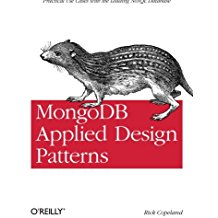
\includegraphics[width=1in]{img/cis-445}} & \hangindent .4in \textbf{Textbook:} Copeland, R. (2013). MongoDB Applied Design Patterns (1st edition). O'Reilly Media. ISBN-10: 1449340040 $\bullet$ ISBN-13: 978-1449340049.
}